% Auriga theme
% https://github.com/anishathalye/auriga
\def\hint{}
\newcommand{\nexthint}[1]{\renewcommand{\hint}{#1}}

\documentclass[14pt,aspectratio=169]{beamer}
\usepackage{pgfpages}
\usepackage{fancyvrb}
\usepackage{tikz}
\usetikzlibrary{tikzmark}
\usepackage{pgfplots}
\usepackage{listings}
\lstset{basicstyle=\small\ttfamily}
\renewcommand{\ttdefault}{pcr}
\usepackage{xcolor}
\usepackage{emoji}
\useoutertheme{miniframes}

\newcommand\refa[1]{{\rmfamily\scshape {#1}}}

\ifnotes
\setbeamertemplate{note page}[plain]
\setbeameroption{show notes on second screen=right}
\fi

\usetheme{auriga}
\usecolortheme{auriga}

% define some colors for a consistent theme across slides
\definecolor{red}{RGB}{181, 23, 0}
\definecolor{blue}{RGB}{0, 118, 186}
\definecolor{gray}{RGB}{146, 146, 146}

\title{A Notion of Equivalence for Refactoring with Abstract Execution\\\scriptsize IFIP WG 1.9/2.15\\31. Oct. 2024}

\author{\underline{Volker Stolz} \inst{1}\vspace{5mm}\\ \and Eduard Kamburjan \inst{2} \and Violet Ka I Pun \inst{1} \and Ole Jørgen Abusdal \inst{1}}

\institute[shortinst]{\inst{1} Western Norway University of Applied Sciences \samelineand \inst{2} University of Oslo}

\begin{document}

{
  \nexthint{Refactoring and Relational Verification}
  % rather than use the frame options [noframenumbering,plain], we make the
  % color match, so that the indicated page numbers match PDF page numbers
  \setbeamercolor{page number in head/foot}{fg=background canvas.bg}
  \begin{frame}
    \titlepage

   \begin{center}
     
\includegraphics[width=2.5cm]{qr.png} ~~~~~ \small
     $\longleftarrow$ For details, see ISoLA'22!
   \end{center}
  \end{frame}
}


% Mention refactoring and relational verification
\section{Intro}
\nexthint{A fundamental relational property} 
\begin{frame}{Refactoring and relational verification} 
  \begin{block}{Refactoring:}
  Improve structure of code, preserve behavior of executions
  \begin{center}
    {\scriptsize \texttt{\textbf{if}(E\tikzmark{OE}) \{S1\tikzmark{OS1};\} \textbf{else} \{S2\tikzmark{OS2};\} \textbf{return};}} \quad \tikzmark{center}\sim \quad {\scriptsize \texttt{\textbf{if}(!E\tikzmark{RE}) \{S2\tikzmark{RS2};\textbf{return};\} S1\tikzmark{RS1}; \textbf{return};}}
    \begin{tikzpicture}[remember picture,overlay]
      \draw (pic cs:center) ++ (0,-8mm) node (root) {\scriptsize placeholders};
      \draw[->,shorten >= 2mm] (root) edge[bend left=25] (pic cs:OS2);
      \draw[->,shorten >= 2mm] (root) edge[bend left=25] (pic cs:OS1);
      \draw[->,shorten >= 2mm] (root) edge[bend right=25] (pic cs:RE);      
    \end{tikzpicture}
  \end{center}
  \end{block}
  \vspace{5mm}
  \begin{block}{Relational verification:}
  Relate pairs of executions, given initial state satisfy $\Phi$ then final state satisfy $\Psi$
  \begin{center}
  $\text{original} \sim \text{refactored} : \Phi \implies \Psi$ 
  \end{center}
  \end{block}
\end{frame}


\nexthint{Relational verification in practice}
\begin{frame}{A fundamental relational property}
\begin{block}{Program equivalence}
  Two programs are equivalent iff they produce the same output when executed on the same input.
\\[2ex]
{\bf Here:} let's look at Java fragments that we consider equivalent.
\end{block}
\vspace{0.5cm}
\begin{itemize}
     \item How far can current tool support take us?
     \item Other definitions of equivalence?
\end{itemize}
% \vspace{0.5cm}

%  See our work in ``Refactoring and Active Object Languages'' from
%  ISoLA'20 for actor languages\ldots

\end{frame}


%%% Local Variables:
%%% mode: plain-tex
%%% TeX-master: "../p"
%%% End:


\section{REFINITY}
\nexthint{Example - slide stm. abstract}
\begin{frame}{Relational verification in practice}
  \begin{block}{REFINITY}
    \begin{itemize}
      \setlength\itemsep{0.5\itemsep}
    \item Built on top of the KeY automated theorem prover
    \item Enables relational verification of ``Java'' with placeholders
    \item Placeholders are subject to Abstract Execution
    \item Has been sufficiently powerful to verify statement level refactorings\footnote{See Dominic Steinhöfel's PhD thesis: \href{Abstract Execution}{https://tuprints.ulb.tu-darmstadt.de/8540/}}
    \end{itemize}
  \end{block}
\end{frame}

\nexthint{Example - slide stm. abs. proved}
\begin{frame}\vspace*{-5mm}
  \begin{center}
    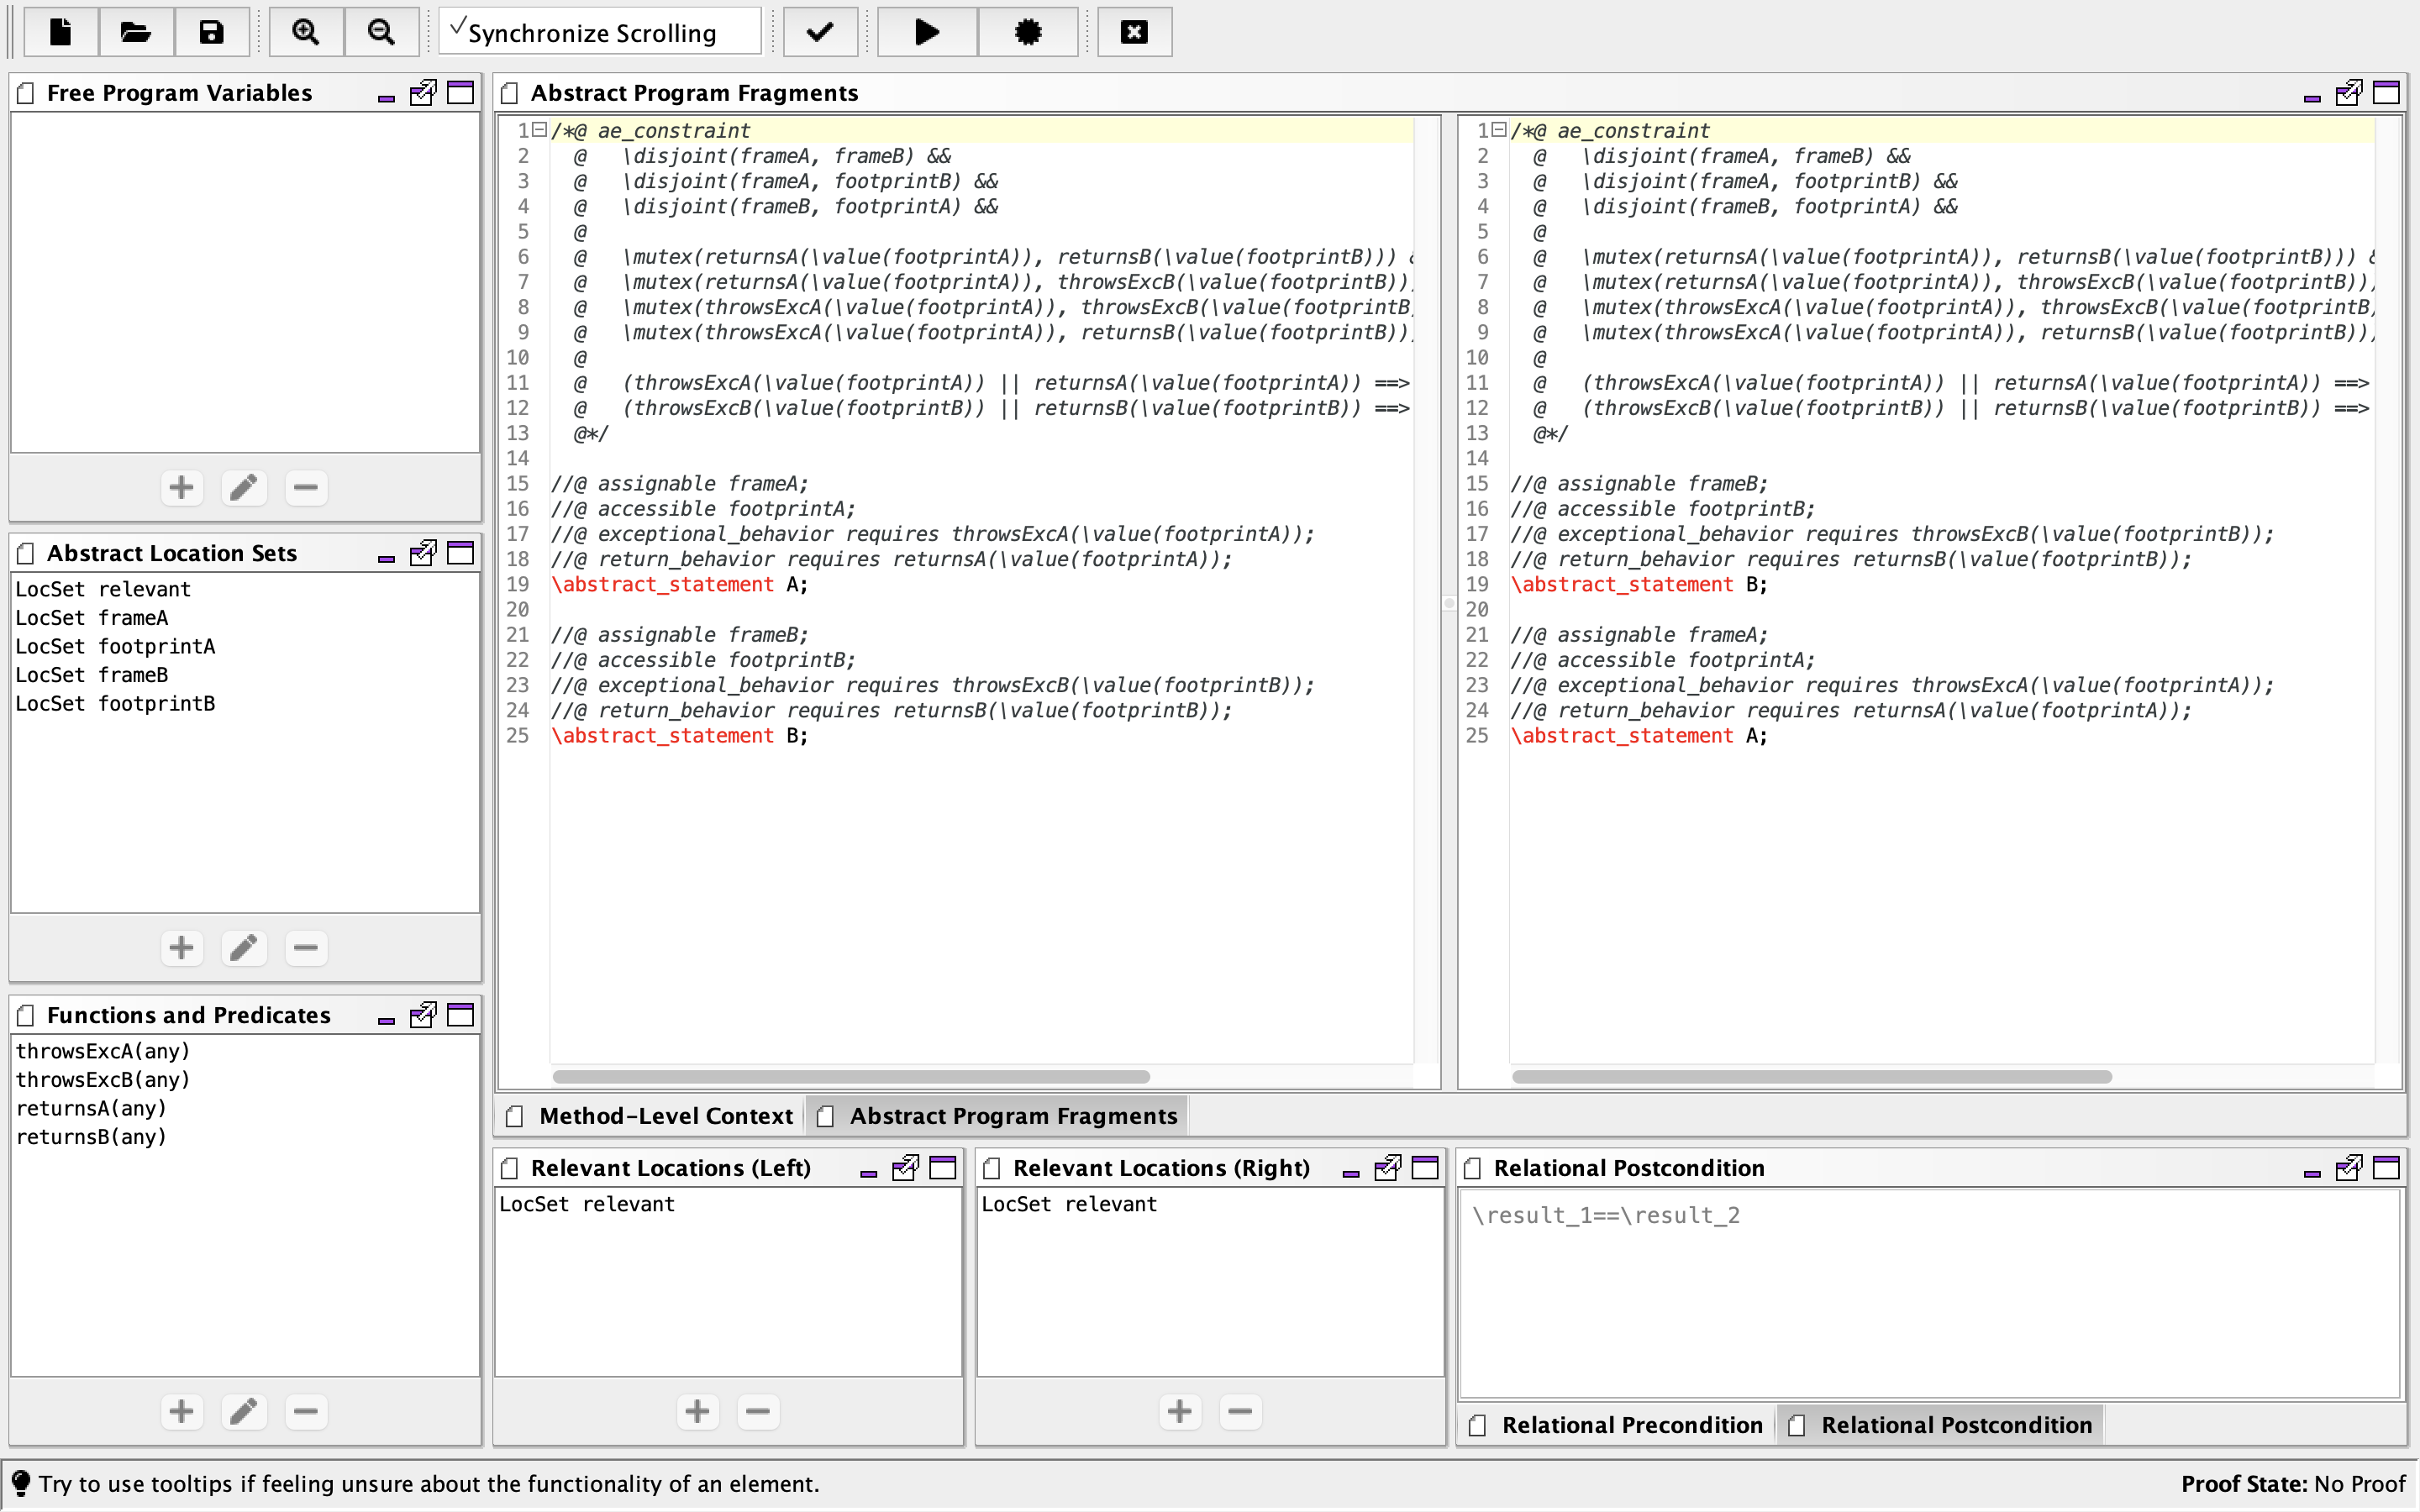
\includegraphics[scale=.25]{screenshots/SlideAbstract}
  \end{center}    
\end{frame}

\nexthint{Example - slide stm. concrete}
\begin{frame}\vspace*{-5mm}
  \begin{center}
    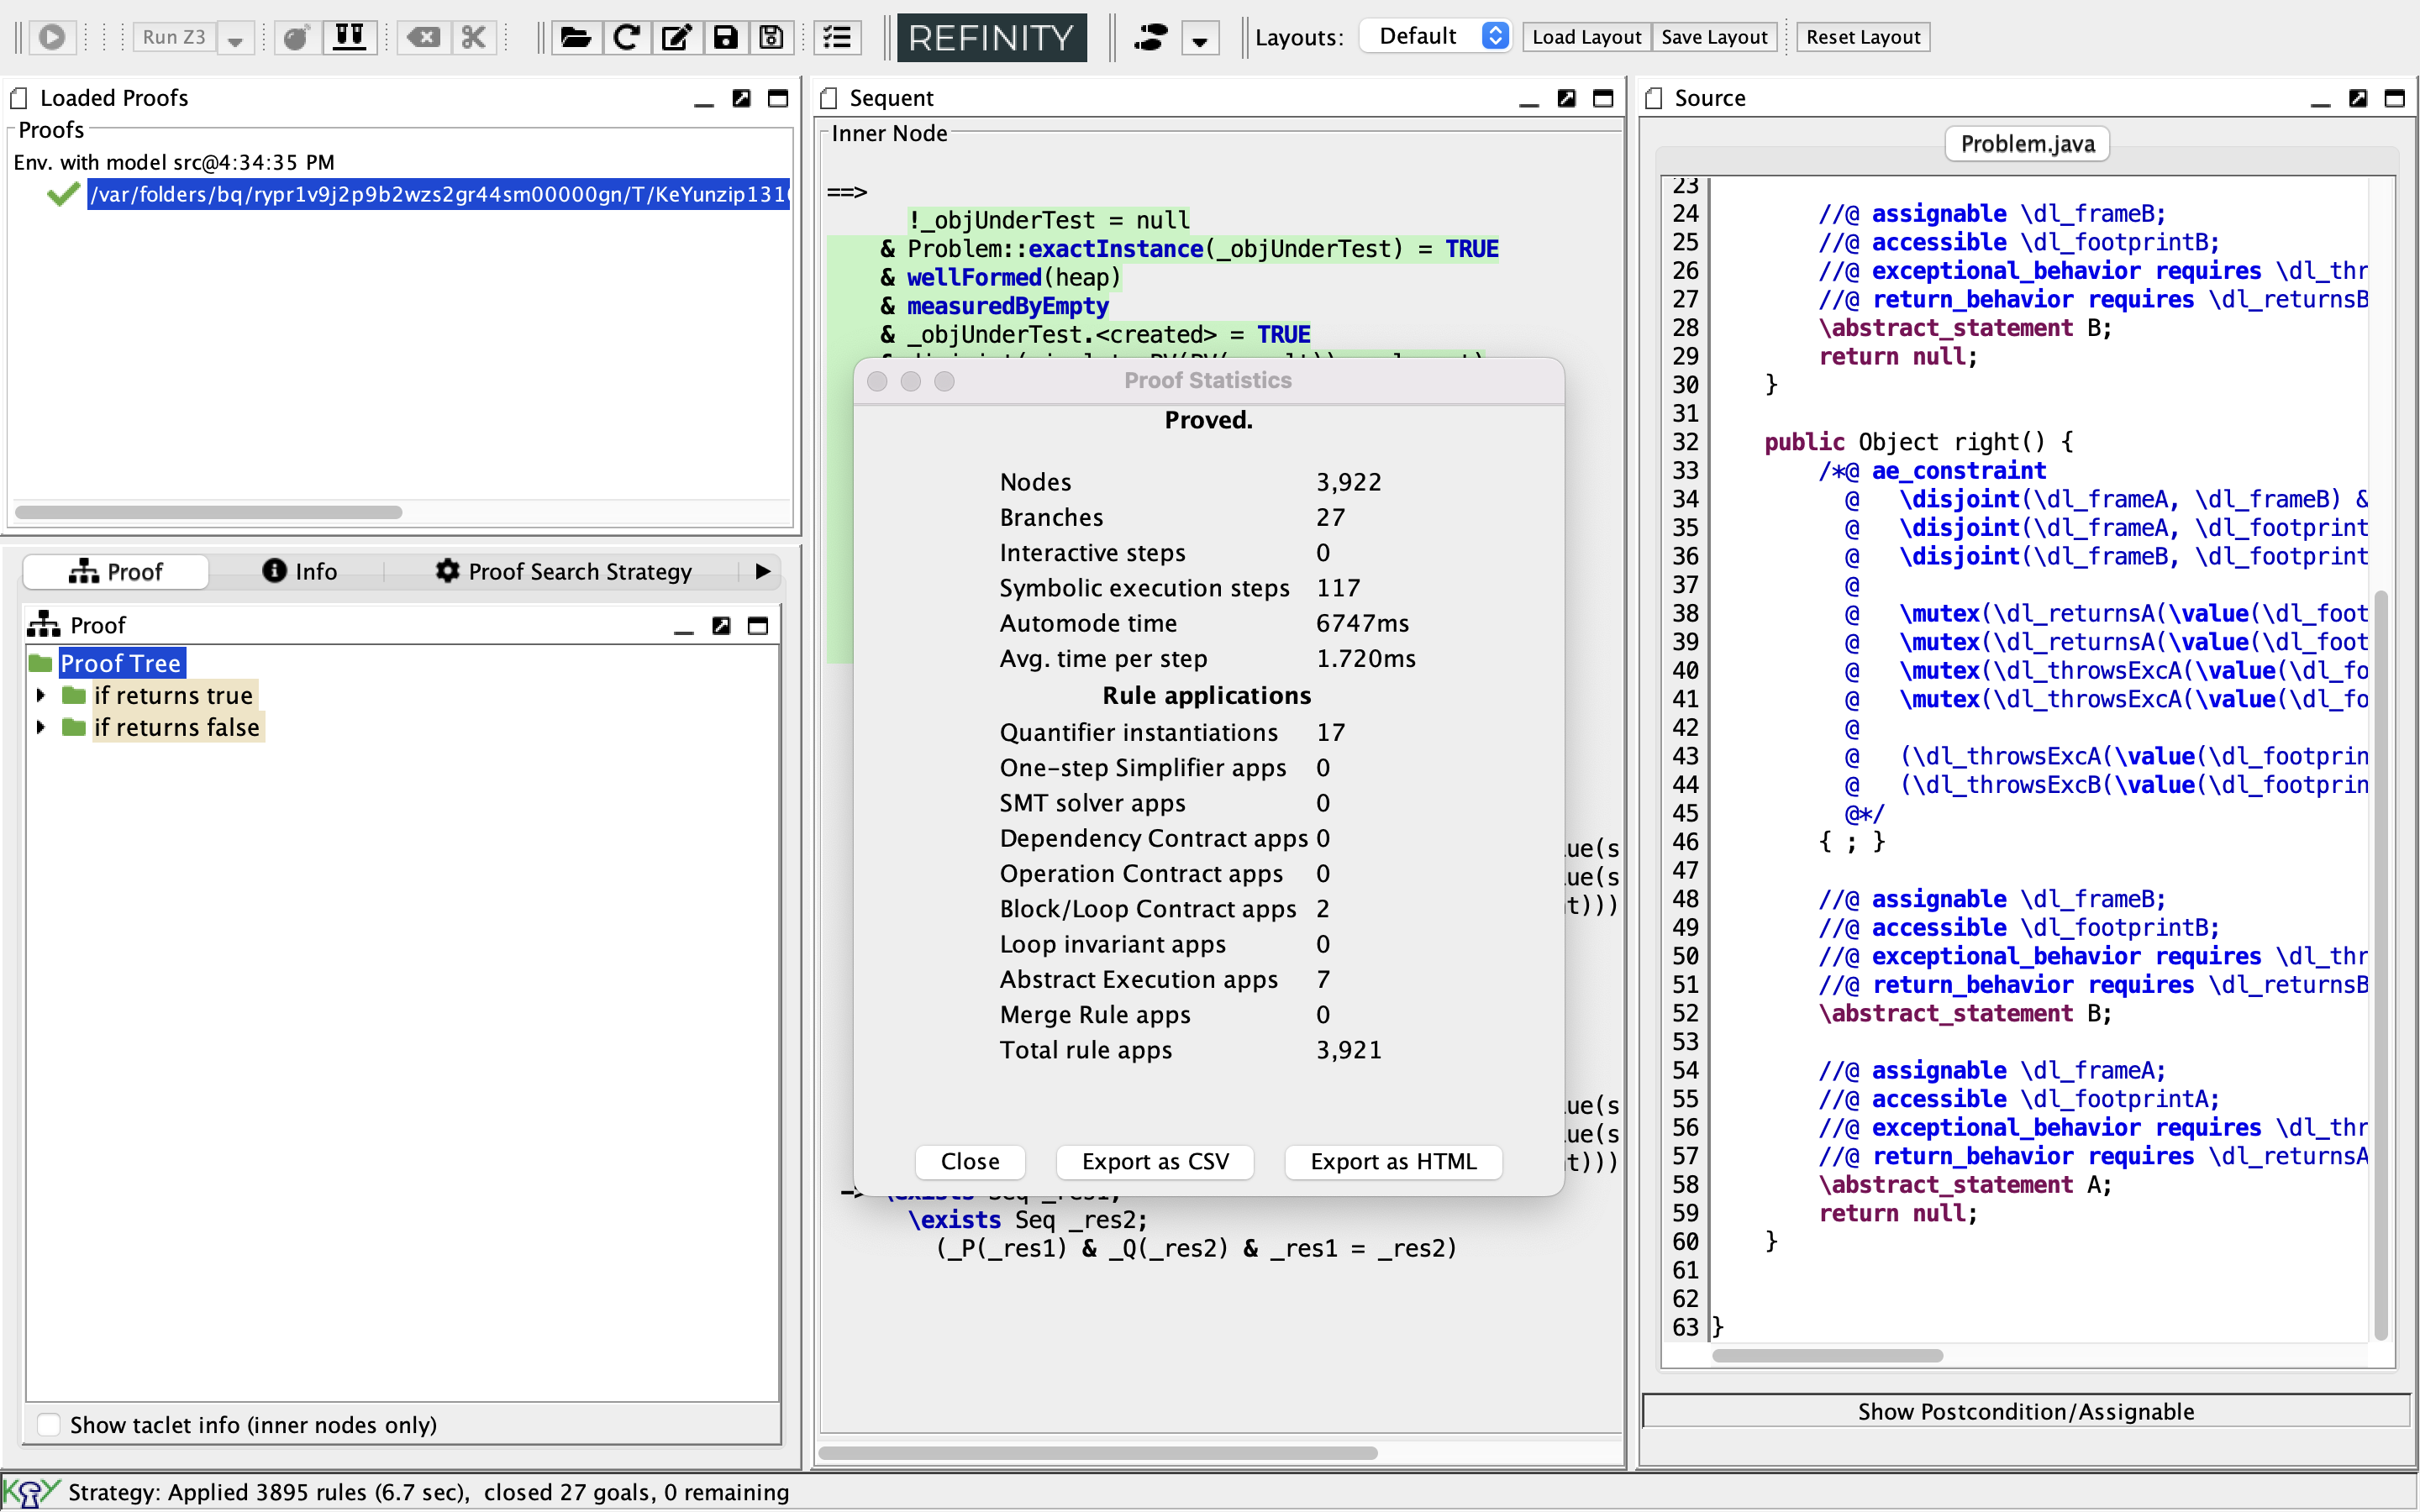
\includegraphics[scale=.25]{screenshots/SlideAbstractProved}
  \end{center}    
\end{frame}

\nexthint{Example - slide stm. conc. open goal}
\begin{frame}\vspace*{-5mm}
  \begin{center}
    \includegraphics[scale=.25]{screenshots/Slide}
  \end{center}    
\end{frame}

\nexthint{Equivalence in REFINITY}
\begin{frame}\vspace*{-5mm}
  \begin{center}
    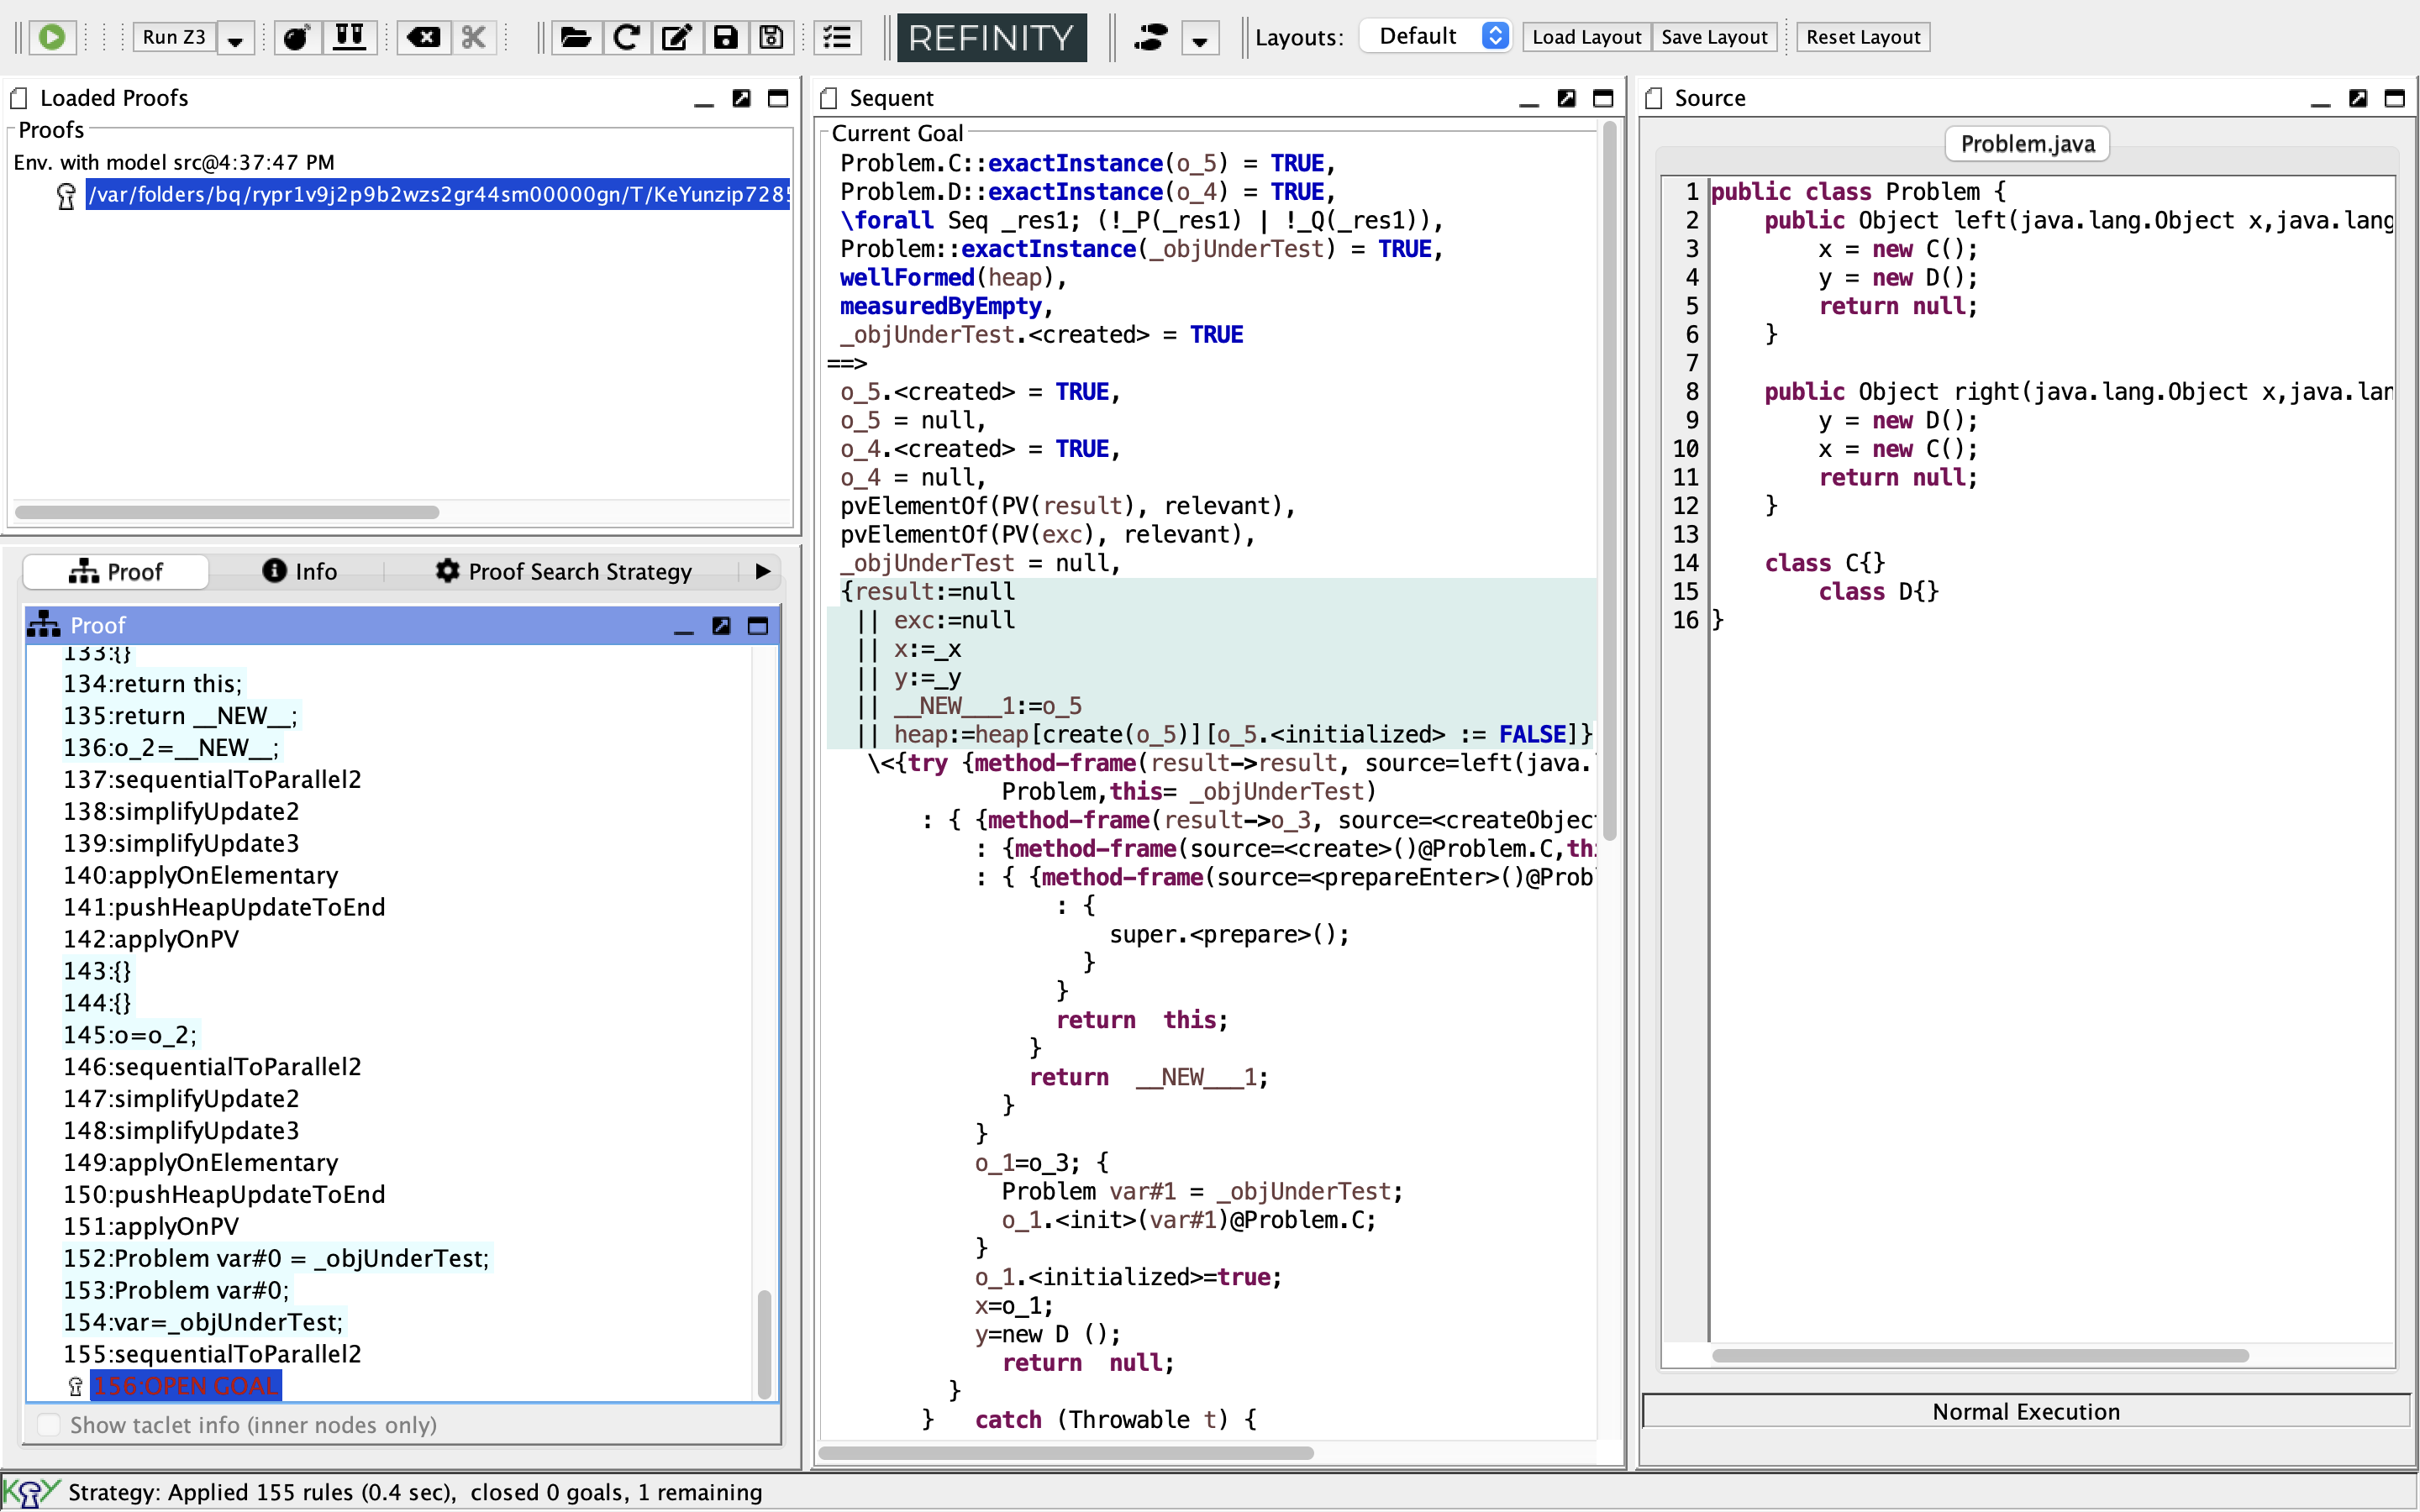
\includegraphics[scale=.25]{screenshots/SlideFail}
  \end{center}    
\end{frame}

\nexthint{Extract Local Variable}
\begin{frame}{Equivalence}
  REFINITY checks that the following are identical by default:
  
  \begin{itemize}
   \item return values
   \item exceptions
   \item objects in the so-called relevant location set
  \end{itemize}
\end{frame}




\nexthint{Example - condition on \lstinline[basicstyle=\tiny]{n()} in REFINITY}
\begin{frame}{Equivalent?}
  Refactoring tools often get this wrong:

\nexthint{Hide Delegate}
\begin{center}
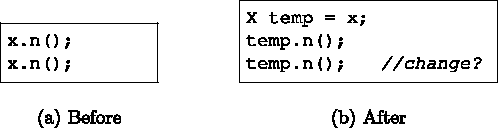
\includegraphics[scale=1.2]{imported/Listing2}
\end{center}

  REFINITY won't close the proof unless you can show the required
  side-conditions on method \lstinline{n()}.

\end{frame}

\nexthint{Hide Delegate}
\begin{frame}\vspace*{-5mm}
  \begin{center}
    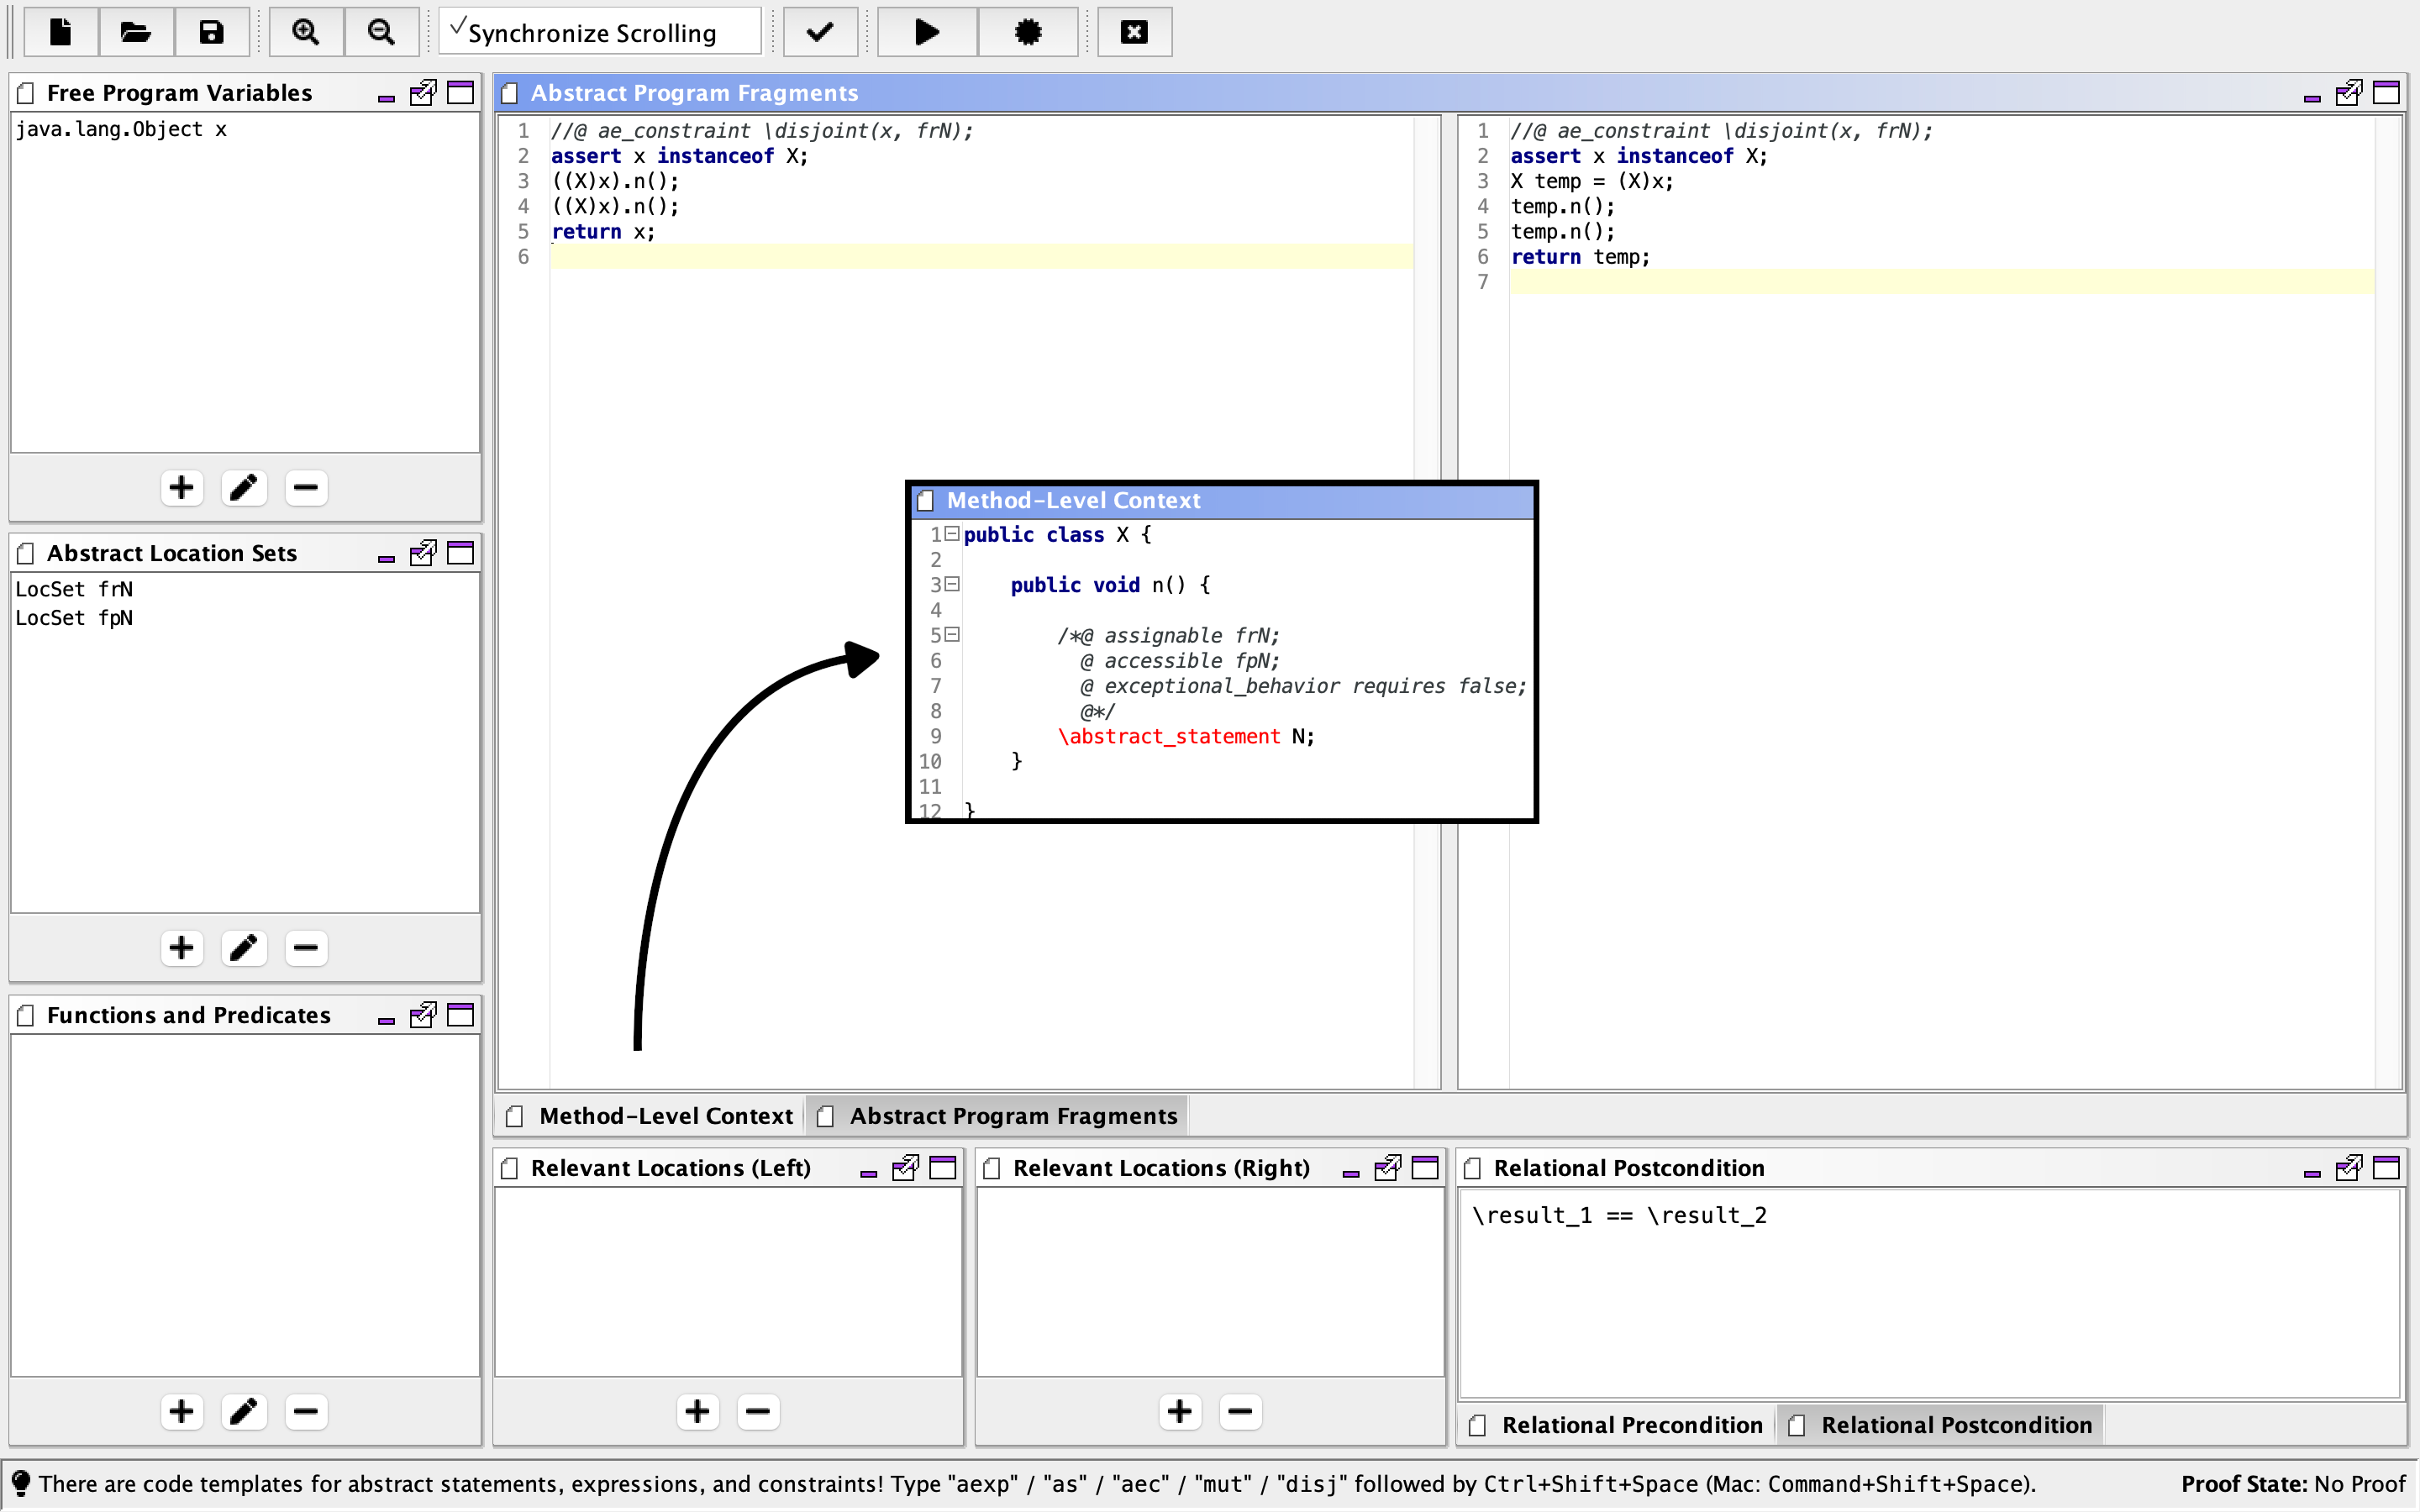
\includegraphics[scale=.25]{screenshots/ExtractLocalVariable}
  \end{center}   
\end{frame}


% \begin{frame}
% \begin{center}
% 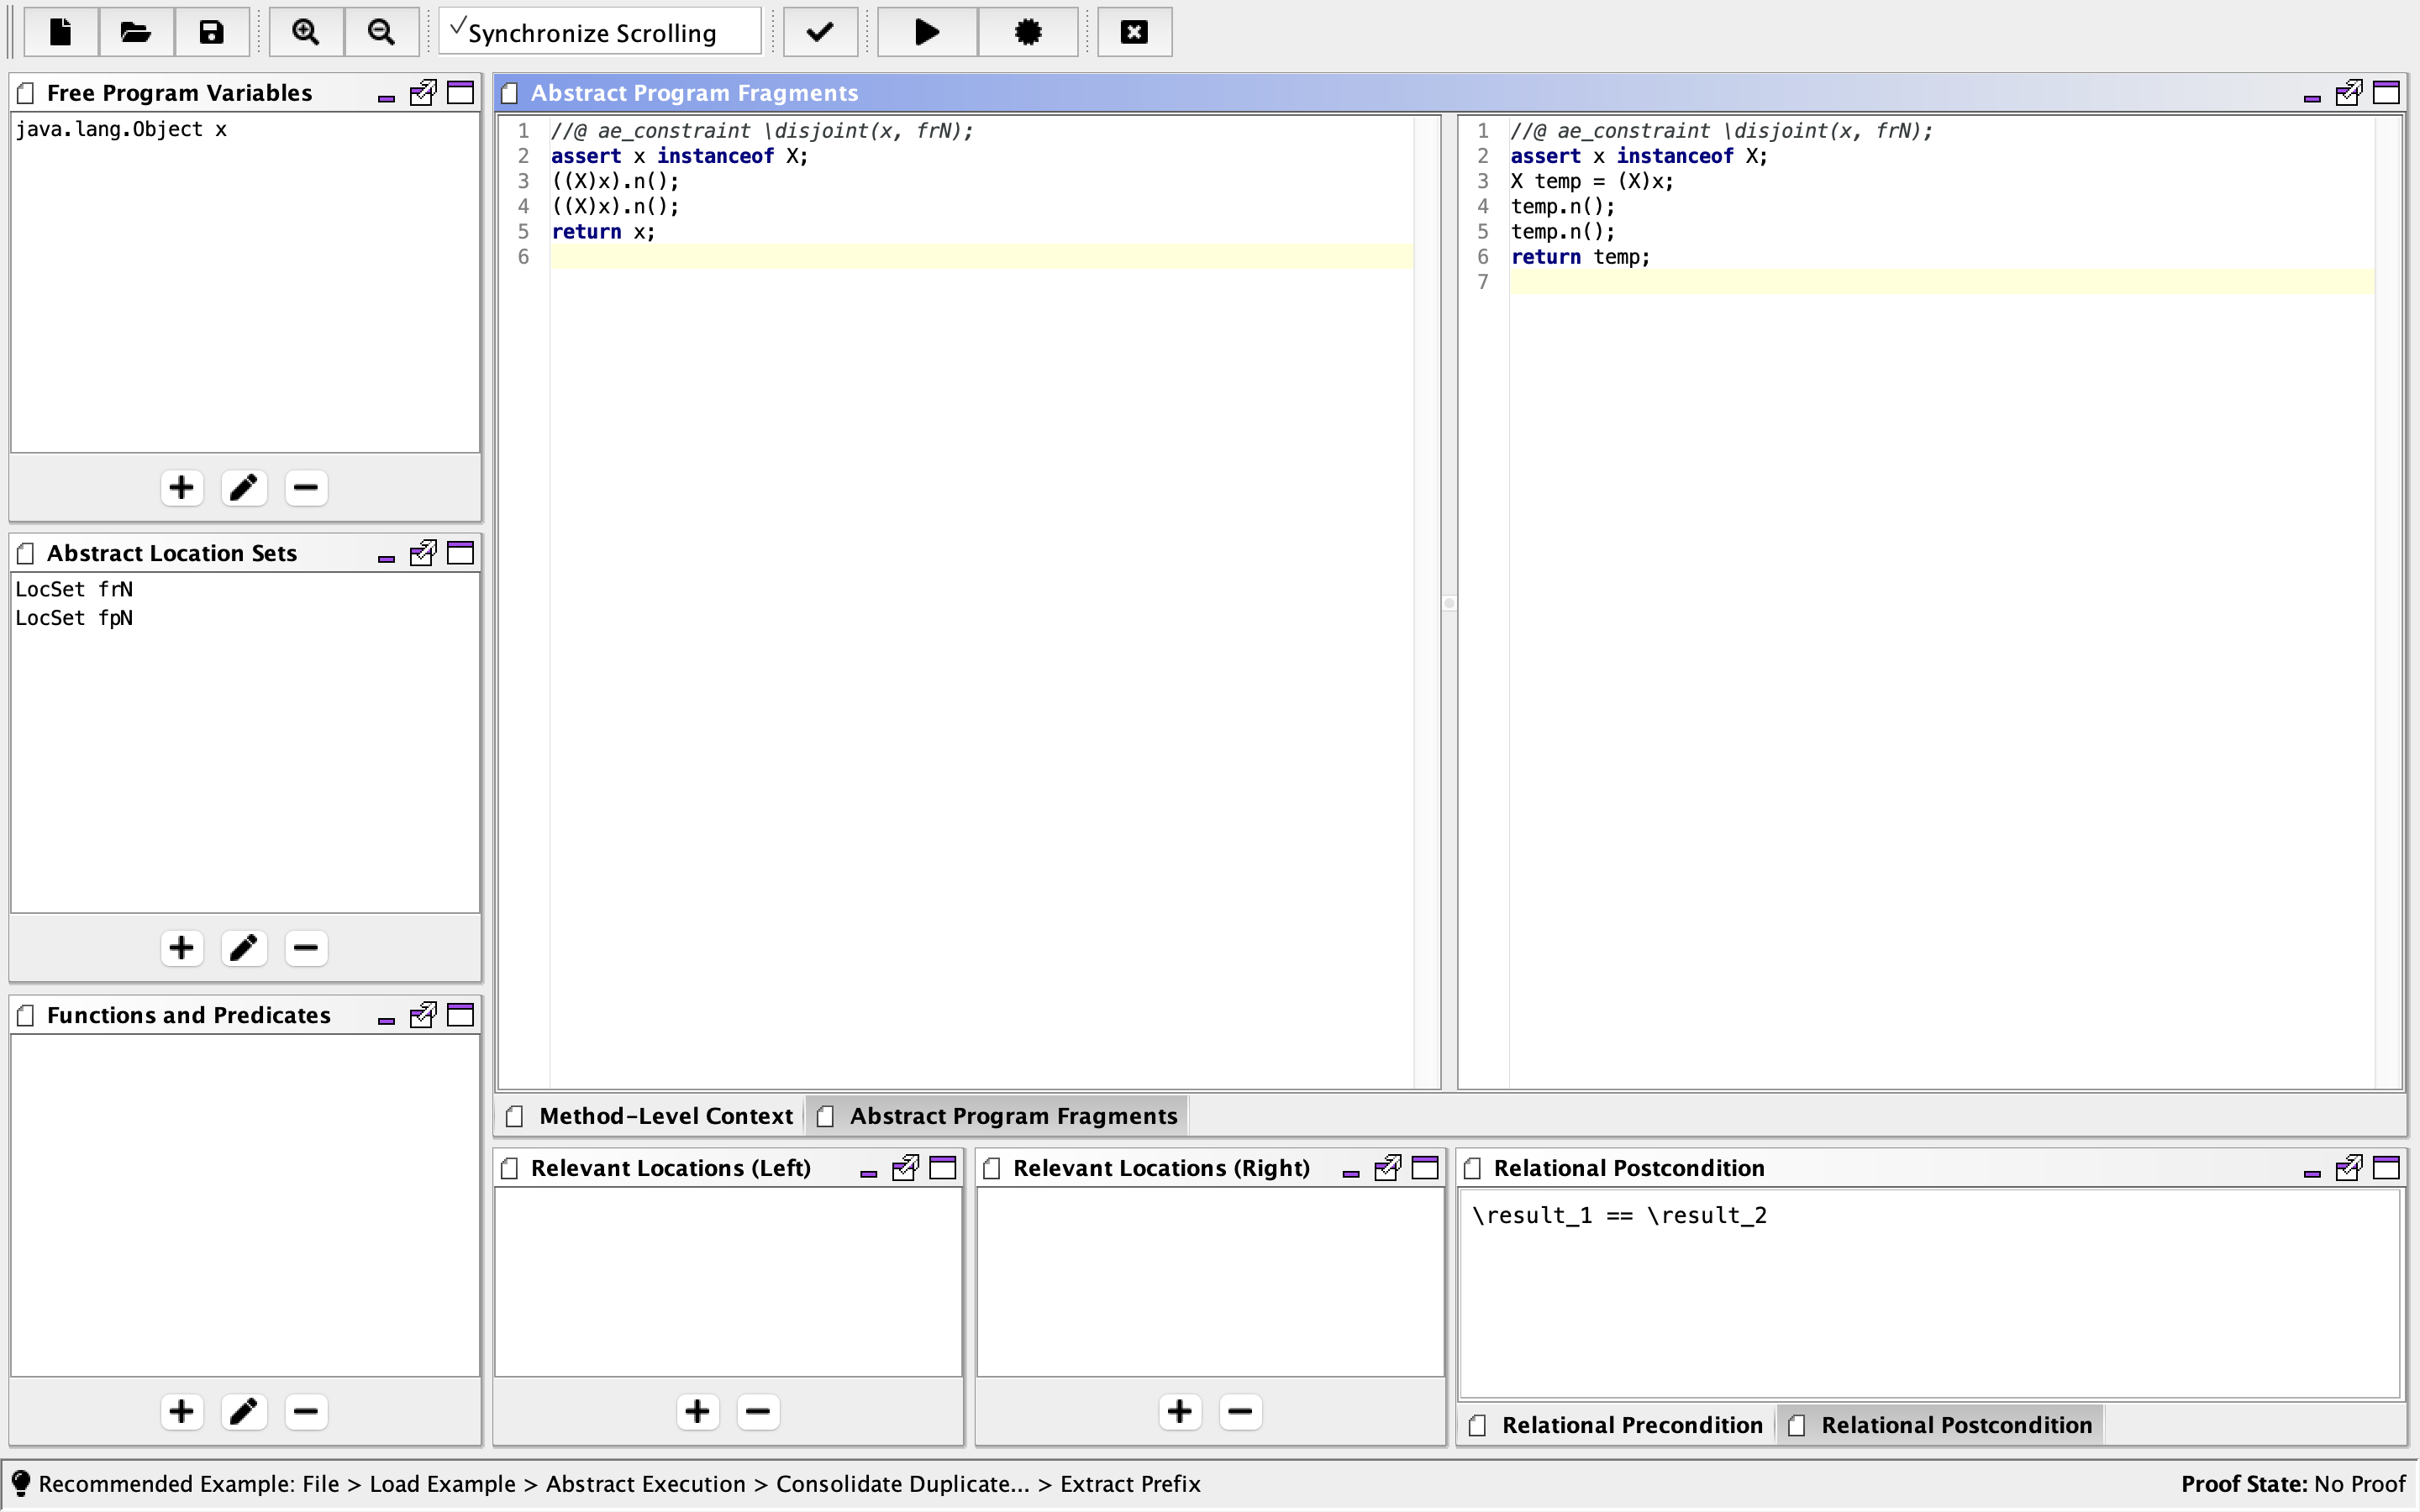
\includegraphics[scale=.26]{screenshots/ExtractVariableAbstract}
% \end{center}  
% \end{frame}

\nexthint{Example - in REFINITY (postcondition)}
\begin{frame}{Different output, but equivalent?}
Exception origin moved, no additional capture in \lstinline{h()}
\vspace{5mm}  
\begin{center}
  \begin{tabular}{rll}
    & \lstinline{o.f().g();}& \\
    $\rightarrow$ & \lstinline{o.h();} & with \lstinline{h()\{ this.f().g();\}}
  \end{tabular}
%{\small \texttt{o.f().g();} $\rightarrow$ \texttt{o.h(); $\mid$ h()\{ this.f().g(); \}}}
\end{center}
\vspace{1mm}       
\begin{minipage}{.49\textwidth}
\begin{figure}
  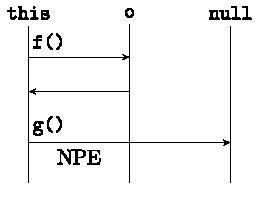
\includegraphics{imported/npe-before}
  \vspace{-1cm}
  \caption{original}
\end{figure}
\end{minipage}
\begin{minipage}{.49\textwidth}
\begin{figure}
  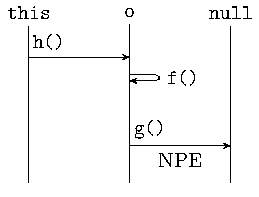
\includegraphics{imported/npe-after}
  \vspace{-1cm}
  \caption{refactored}
\end{figure}
\end{minipage}
\end{frame}

\nexthint{Challenges}
\begin{frame}\vspace*{-5mm}
\begin{center}
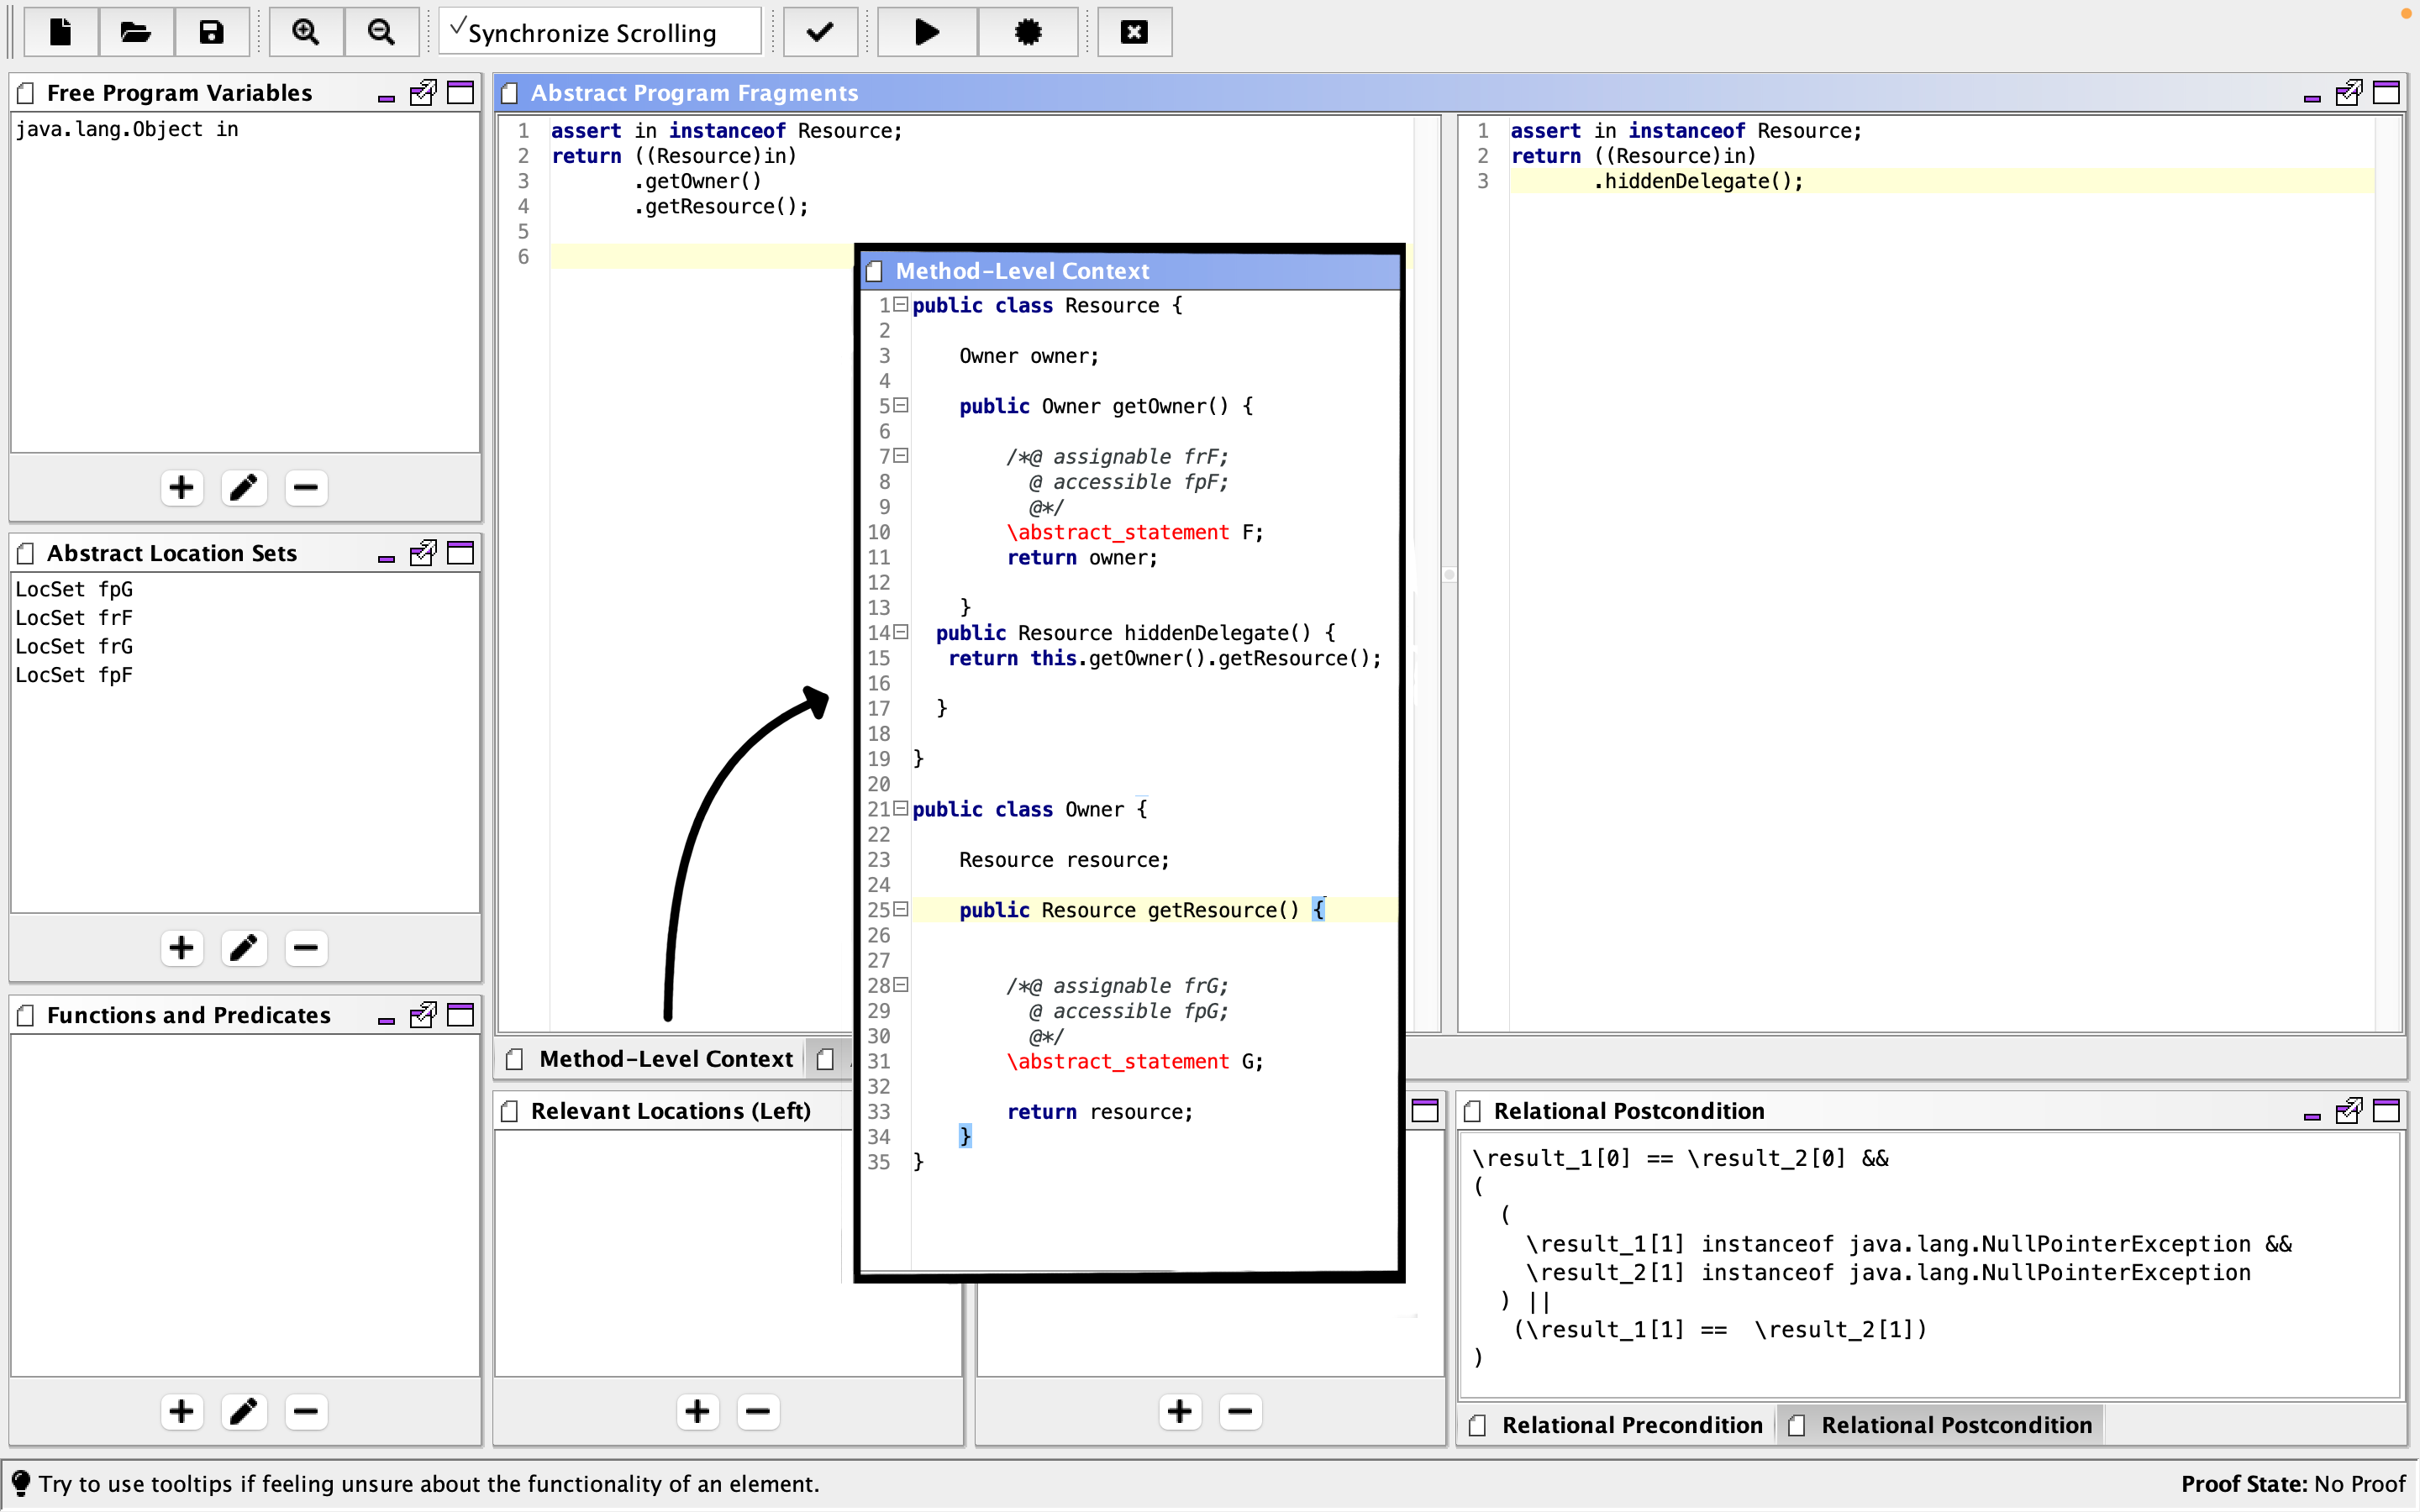
\includegraphics[scale=.25]{screenshots/HideDelegateAbstract}
\end{center}
\end{frame}

\nexthint{Object equality I}
\begin{frame}{Challenges in complex refactorings}
  Succesfully verified variants of \textit{Extract Local Variable} and \textit{Hide Delegate} and investigated how to approach others.
  \begin{block}{We discuss}
  Simplifying postcondition specifications
  \end{block}
  \begin{block}{Unresolved}
    Making the proofs useful artefacts:\\
    what about \emph{instantitations}?
  \end{block}
\end{frame}



% Go through how the object  problem was tackled
\section{Object Creation}
\nexthint{Example - Slide stm. abs.}
\begin{frame}{Object equality}
REFINITY lacked rules for object equality over multiple modalities:
\begin{itemize}
\item can verify \refa{Slide Statement} with abstract statements
\end{itemize}
\end{frame}

\nexthint{Object equality II}
\begin{frame}\vspace*{-5mm}
\begin{center}
  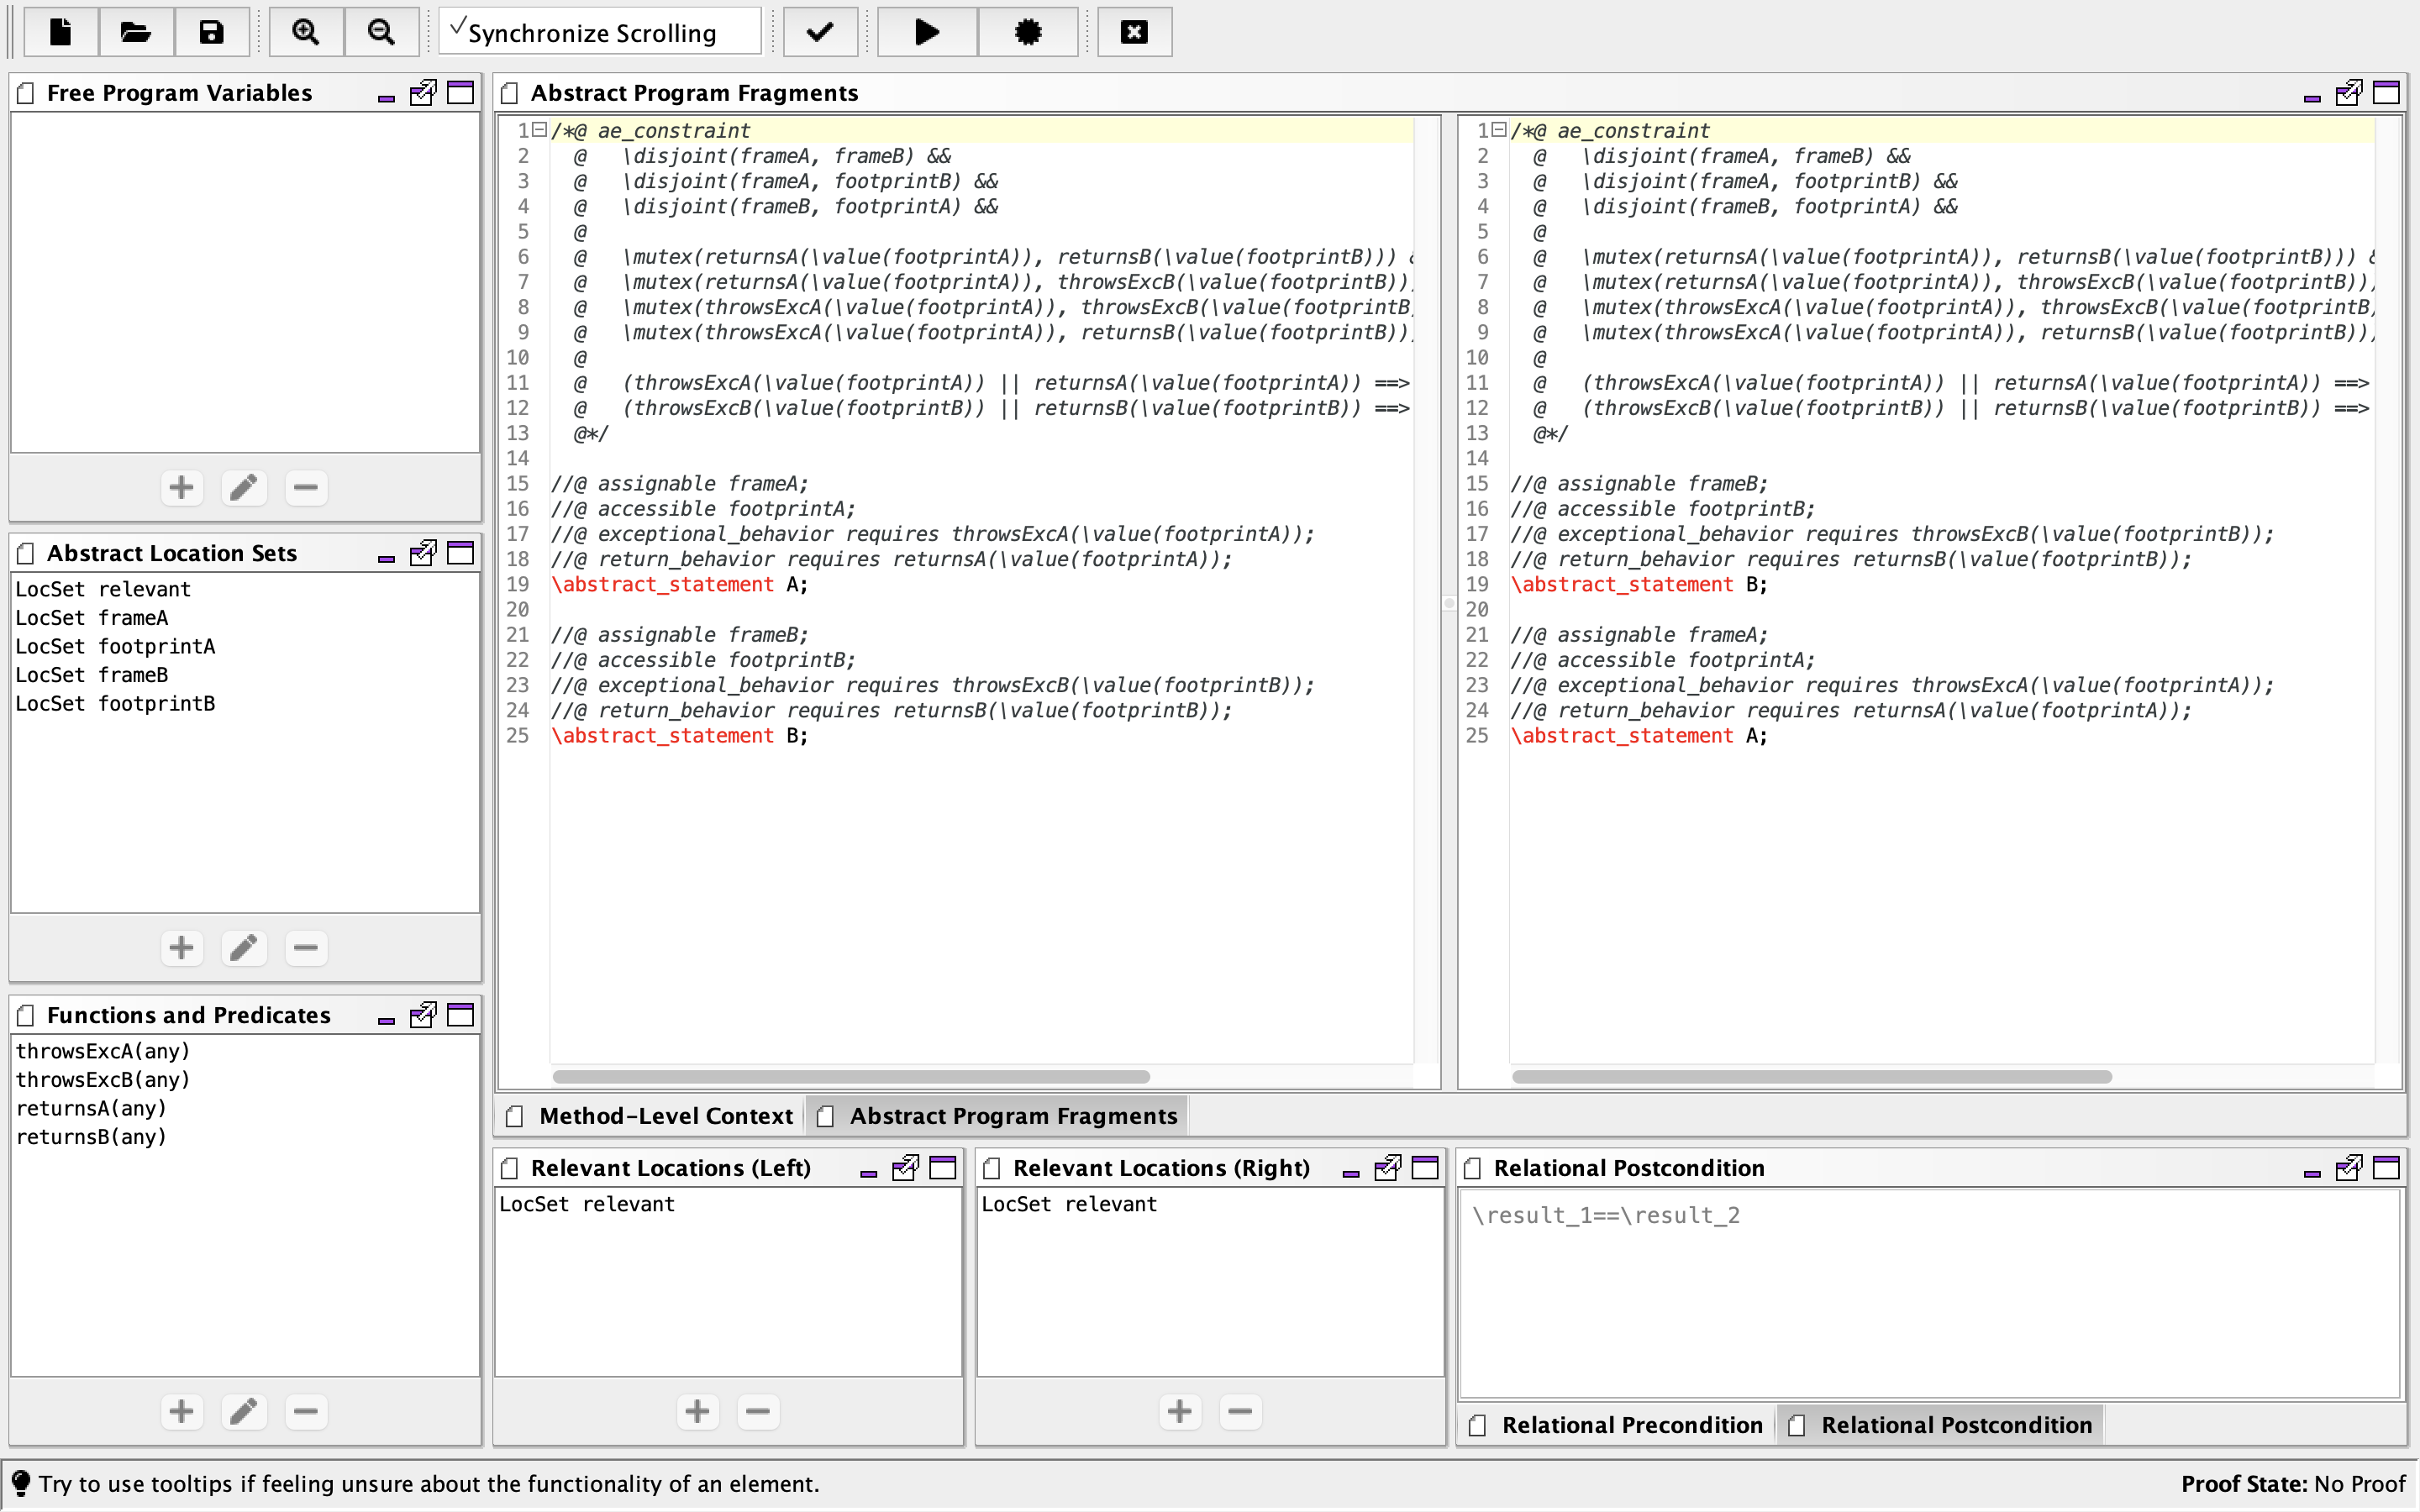
\includegraphics[scale=.25]{screenshots/SlideAbstract}
\end{center}
\end{frame}

\nexthint{Example - Slide stm. conc.}
\begin{frame}{Object equality}
REFINITY lacked rules for object equality over multiple modalities:
\begin{itemize}
\item can verify Slide Statement with abstract statements
\item can't verify Slide Statement with statements involving concrete objects
\end{itemize}
\end{frame}

\nexthint{Why?}
\begin{frame}\vspace*{-5mm}
\begin{center}
  \includegraphics[scale=.25]{screenshots/Slide}
\end{center}
\end{frame}

\nexthint{Adding taclets and rules}
\begin{frame}{REFINITY Internals}
  Core issue:
  \begin{itemize}
    \item Objects are placed in a symbolic heap during SE
    \item Before and After program executed in same proof
    \end{itemize}

\medskip    
Not sufficient for two new objects to be equal:
  \begin{itemize}
    \item the allocation must, additionally, be deterministic
  \end{itemize}
\end{frame}


%taclets
%They contain the declarative, logical content of the rule schemata, but also pragmatic information:
%in which context and when a rule should be applied by an automated reasoning strategy and how it is to be presented to the user.
%At the core of the KeY system is an efficient interpreter that applies taclets to goal sequents and thereby constructs proof trees.
\nexthint{Definition 1}
\begin{frame}{Adding rules required for object equality}
  Schematic sequent rules in KeY are specified as \textit{taclets}:
  \begin{itemize}
  \item we add rules to make objects indistinguishable under under certain conditions
  \end{itemize}
\end{frame}

\nexthint{Definition 2}
% \begin{frame}
%   \begin{center}
%   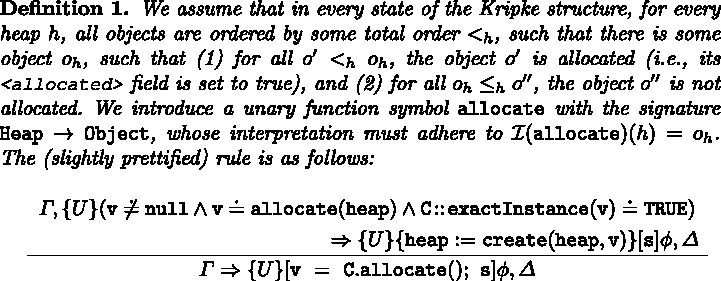
\includegraphics{imported/Definition1}
%   \end{center}
% \end{frame}

\nexthint{Postcondition simplification}
\begin{frame}{New \textit{taclet} for object creation}
  \begin{center}
  \includegraphics[width=\linewidth]{imported/Definition2}
  \end{center}
\end{frame}

\nexthint{Example - Hide Delegate (default postcondition)}
\begin{frame}{Postcondition simplification}
In \refa{Hide Delegate} exception objects now equivalent
\begin{itemize}
  \item we need no special postcondition to handle exceptions\ldots
    \item \ldots although we should because in practice exceptions
      capture state! {\small (Not \emph{our} problem, though \emoji{upside-down-face})}
  \end{itemize}
\end{frame}

\nexthint{Future challenges}
\begin{frame}\vspace*{-5mm}
  \begin{center}
  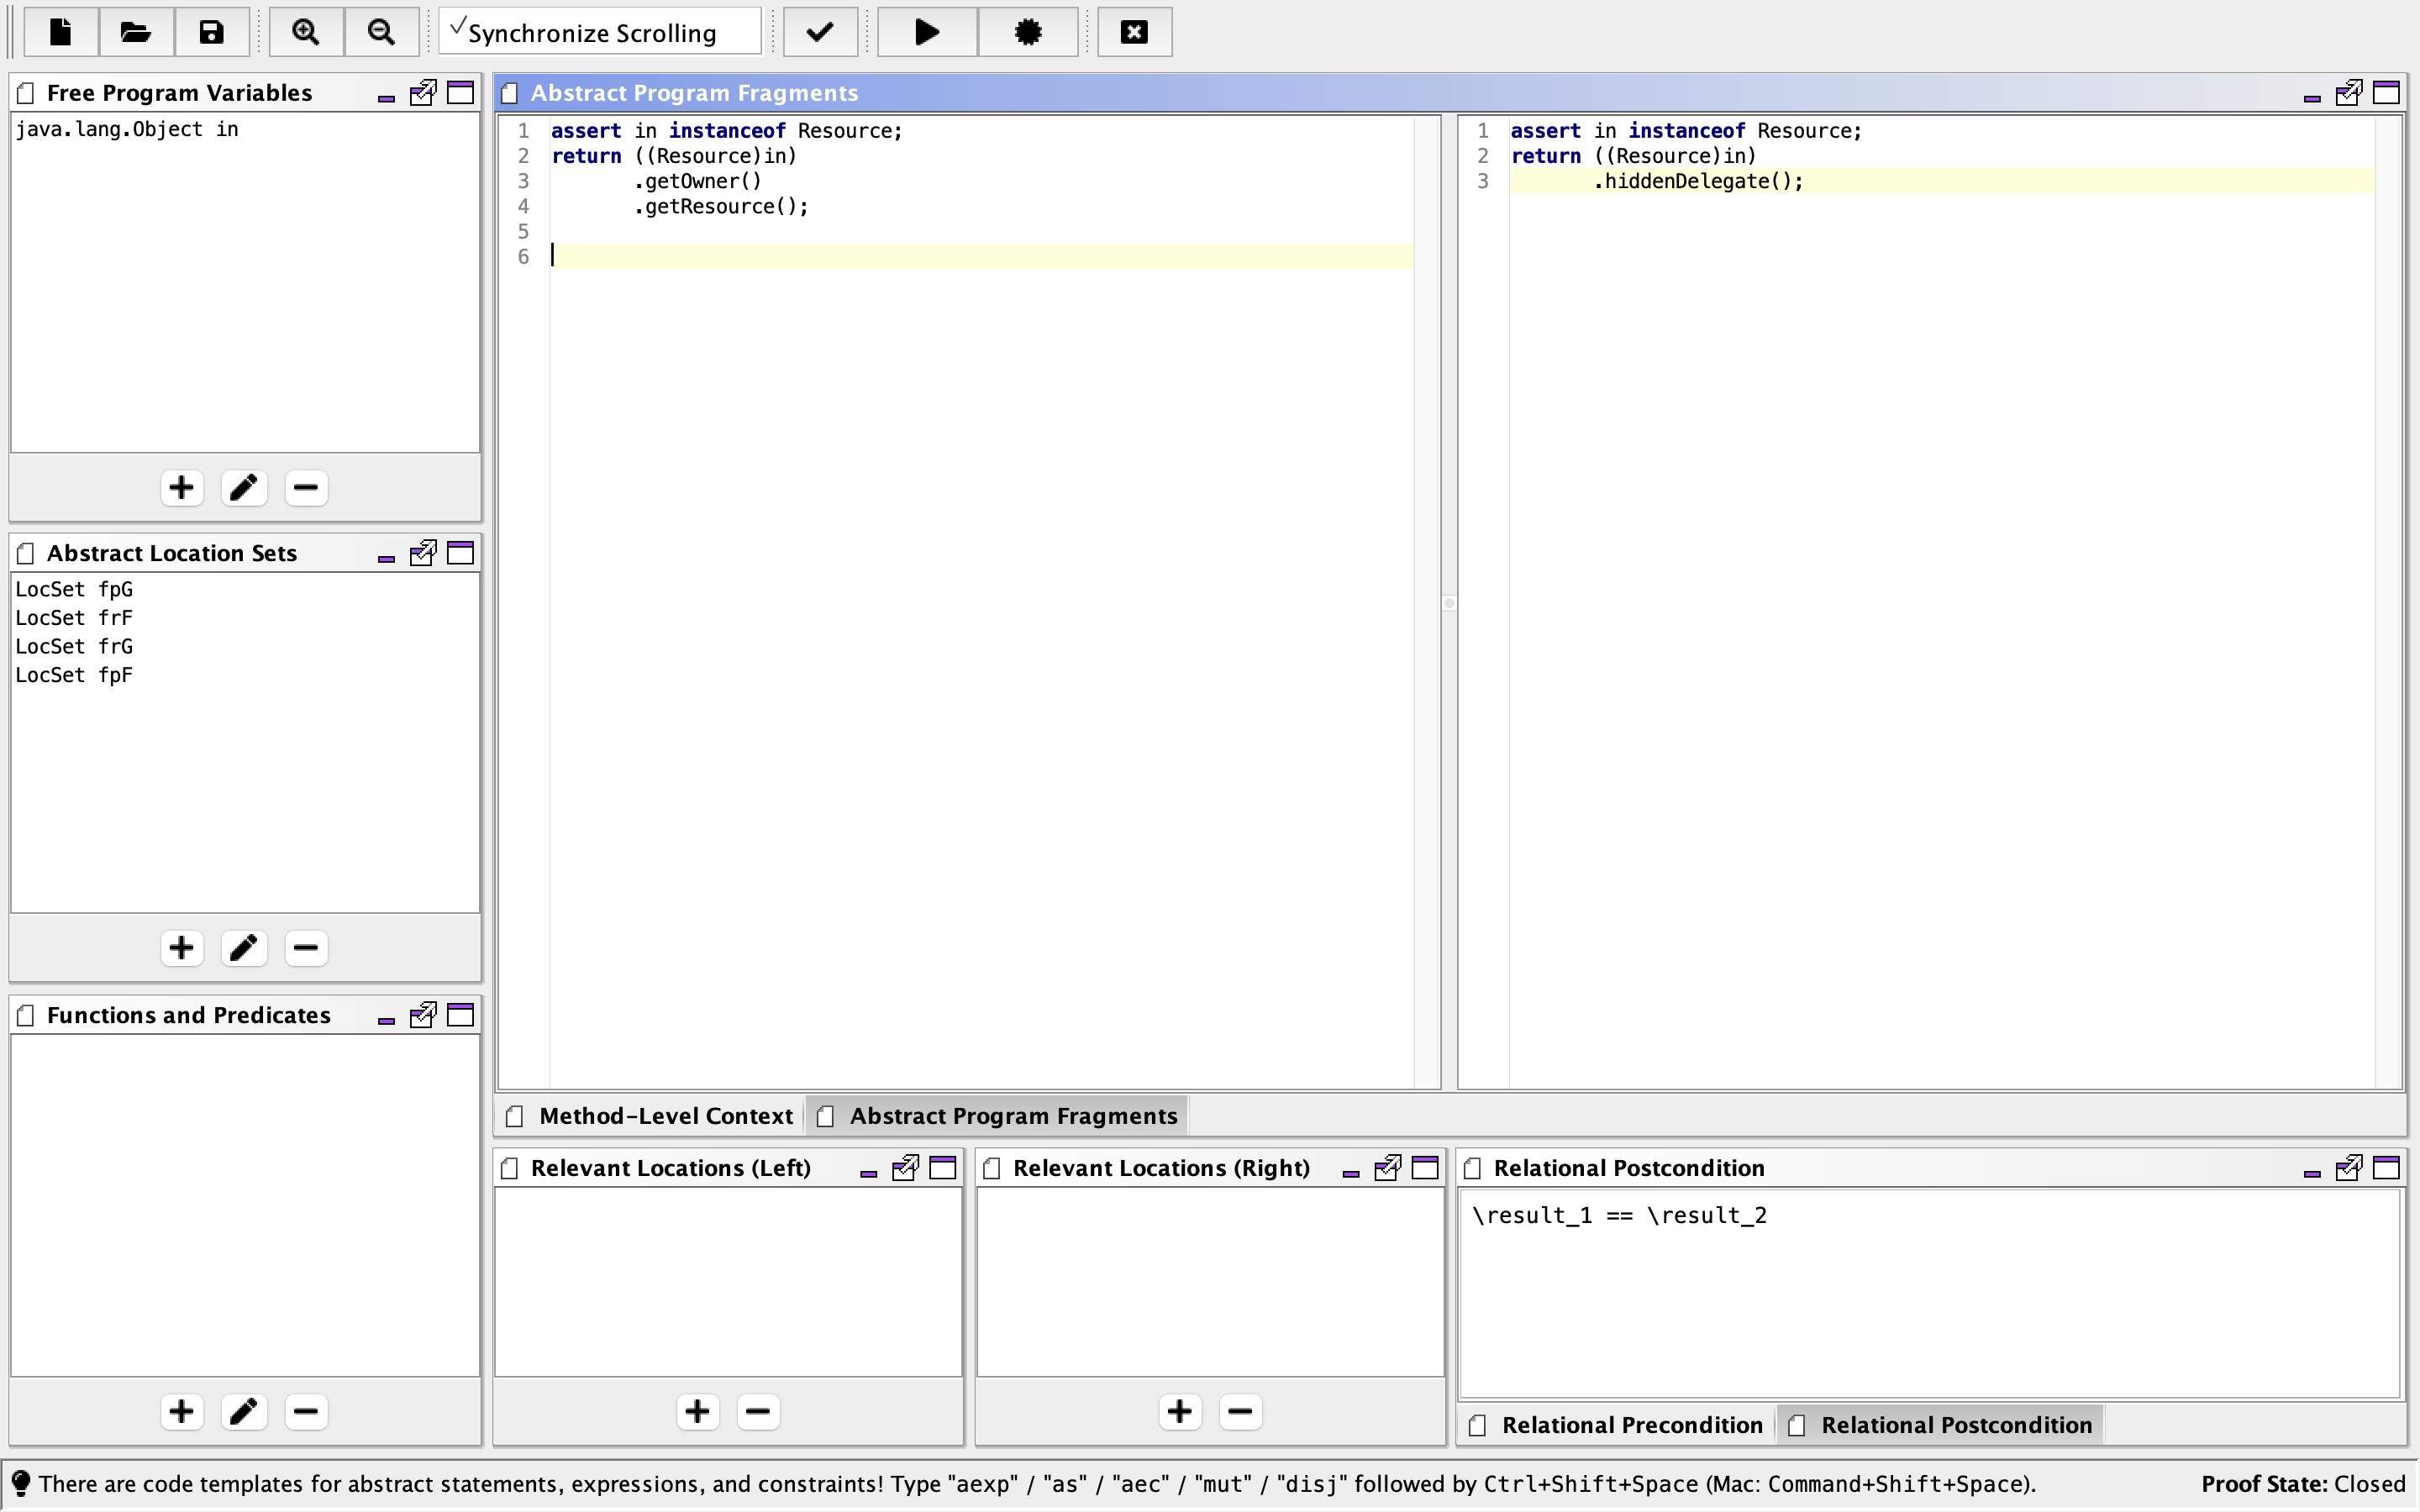
\includegraphics[scale=0.25]{screenshots/HideDelegateDefaultPostcondition}
  \end{center}
\end{frame}



% The wishful thinking bits: substitute datastructure, mention trace properties for the 
\section{Future Challenges}
\begin{frame}
  \vfill
  \begin{center}
  { \Huge Future Challenges }
  \end{center}
  \vfill
\end{frame}

\nexthint{Trace based notions of equivalence}
\begin{frame}{Dead code/object removal}
  \begin{center}
  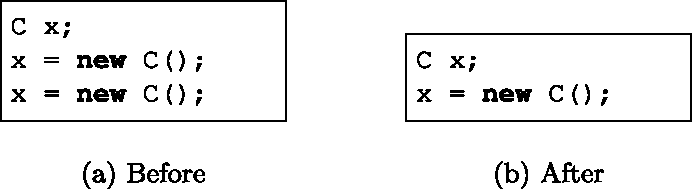
\includegraphics{imported/Listing8}
  \end{center}
\end{frame}

\nexthint{Substitute data structure}
\begin{frame}{Trace based notions of equivalence}
  \begin{center}
  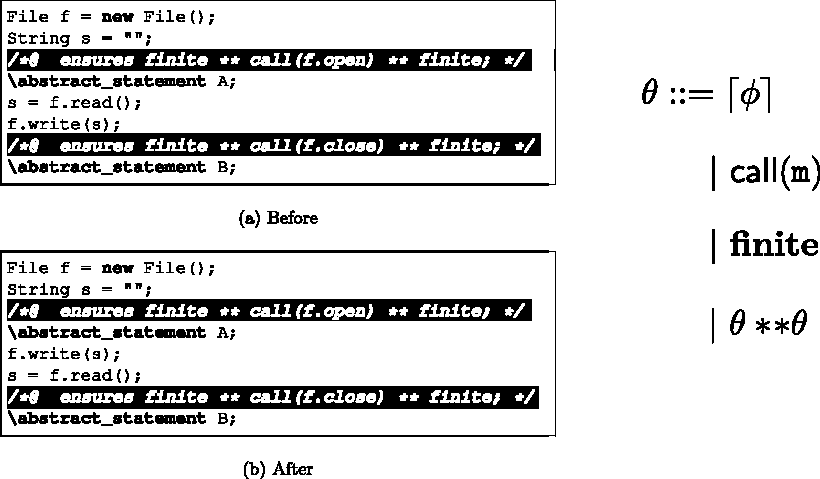
\includegraphics[scale=.8]{imported/Traces-thick}
  \end{center}
\end{frame}

\nexthint{Questions?}
\begin{frame}{Substitute data structure}
  \begin{center}
  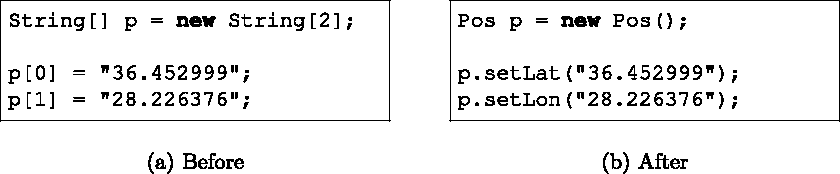
\includegraphics{imported/Listing10}
  \end{center}
\end{frame}


\begin{frame}
  \frametitle{Summary}

  \begin{itemize}
  \item REFINITY/KeY excellent foundation
  \item Contributed a few more example refactoring:\\
    \refa{Extract Local Variable}, \refa{Hide Delegate}\\[-7ex]
  \item[] 
    \begin{itemize}
    \item abstract code + side conditions
    \item needed more taclets for proof support on the way
    \end{itemize}
  \item To Do:
    \begin{itemize}
    \item more intermediate taclets (e.g.\ for dead code)
    \item more refactorings (within our means)
    \end{itemize}
  \end{itemize}
\end{frame}



\end{document}
